%% Author_tex.tex
%% V1.0
%% 2012/13/12
%% developed by Techset
%%
%% This file describes the coding for rsproca.cls

\documentclass[openacc]{rsproca_new}%%%%where rsproca is the template name
\usepackage{subcaption}
\usepackage[thinc]{esdiff} % for derivatives
\usepackage{empheq} % boxed equations
\usepackage{amsmath}
%\usepackage[section]{placeins}


\definecolor{myboxcolor}{rgb}{0.96, 0.96, 0.96}
\newcommand*\mybox[1]{%
\colorbox{myboxcolor}{\hspace{1em}#1\hspace{1em}}}

\usepackage{xspace}
\newcommand\thedata {$\{(t_i,h_{\text{obs}, i})\}_{i=1}^{N}$\xspace}
\newcommand\thedatanomath {\{(t_i,h_{\text{obs}, i})\}_{i=1}^{N}}
\newcommand\themodel {$h(t; h_0, \boldsymbol \alpha, \boldsymbol\theta)$\xspace}
\newcommand\themodelnomath {h(t; h_0, \boldsymbol \alpha, \boldsymbol\theta)}
\newcommand\thevars{h_0, \boldsymbol \alpha, \boldsymbol \theta, \sigma^2}
\newcommand\thesamples{$(h_{0, i}, \boldsymbol \alpha_i, \boldsymbol \theta_i, \sigma_i^2)_{i=1}^{N_s}$}



% from empheq pkg
\definecolor{shadecolor}{rgb}{0.97, 0.97, 1.0}
\definecolor{titlecolor}{rgb}{0.96, 1.0, 0.98}
\newsavebox{\mysaveboxM} % M for math
\newsavebox{\mysaveboxT} % T for text
\newcommand*\Garybox[2][Example]{%
\sbox{\mysaveboxM}{#2}%
\sbox{\mysaveboxT}{\fcolorbox{black}{titlecolor}{#1}}%
\sbox{\mysaveboxM}{%
\fcolorbox{black}{shadecolor}{%
\makebox[\linewidth-10em]{\usebox{\mysaveboxM}}%
}%
}%
\usebox{\mysaveboxM}%
\makebox[0pt][r]{%
\makebox[\wd\mysaveboxM][c]{%
\raisebox{\ht\mysaveboxM-0.5\ht\mysaveboxT
+1.6\dp\mysaveboxT-0.5\fboxrule}{\usebox{\mysaveboxT}}%
}%
}%
}


\usepackage{tcolorbox} 
\tcbuselibrary{breakable}
\newtcolorbox[auto counter
]{mytcbox}[2][]{
% title=Box~\thetcbcounter: #2,#1,
title=#2, #1,
colback=white,
colframe=black,
fonttitle=\bfseries,
parbox=false
}


%%%% *** Do not adjust lengths that control margins, column widths, etc. ***

%%%%%%%%%%% Defining Enunciations  %%%%%%%%%%%
\newtheorem{theorem}{\bf Theorem}[section]
\newtheorem{condition}{\bf Condition}[section]
\newtheorem{corollary}{\bf Corollary}[section]
%%%%%%%%%%%%%%%%%%%%%%%%%%%%%%%%%%%%%%%%%%%%%%%

%%%%% Please insert respective article type here %%%%
\titlehead{Research}

\begin{document}

%%%% Article title to be placed here
% \title{Bayesian inference of the shape of an object inside of a gravity-drained tank}
%\title{Inferring the shape of a solid inside a gravity-drained tank from liquid level time series data}
\title{Inferring the shape of a solid inside a draining tank from liquid level dynamics}


\author{%%%% Author details
Gbenga Fabusola$^{1}$, 
Cory M. Simon$^{1}$
}

%%%%%%%%% Insert author address here
\address{$^{1}$School of Chemical, Biological, and Environmental Engineering. Oregon State University. Corvallis, OR, USA.
% $^{2}$Second author address\\
}

%%%% Subject entries to be placed here %%%%
\subject{applied mathematics, chemical engineering}

%%%% Keyword entries to be placed here %%%%
\keywords{inverse problems, Bayesian statistical inversion, Torricelli's law}

%%%% Insert corresponding author and its email address}
\corres{Cory M. Simon\\
\email{cory.simon@oregonstate.edu}}

%%%% Abstract text to be placed here %%%%%%%%%%%%
\begin{abstract}
In engineering, we often encounter an open-top, liquid-holding tank draining via gravity-driven flow through a small orifice in its side. 
Torricelli's law and a mass balance give a differential equation model governing the dynamics of the liquid level in such a draining tank. 
Herein, we leverage this forward model to tackle an inverse problem of reconstruction: infer the shape of an exogenous, heavy solid inside a draining tank from measurements of its liquid level over time. To quantify uncertainty, we employ Bayesian statistical inversion to obtain a posterior distribution over the solid's cross-sectional area as a function of height. 
(Because the solid displaces liquid, the rate of decrease of the liquid level provides information about the cross-sectional area of the solid at that height; 
as the liquid level drops, it ``scans'' the area of the solid as a function of height.) 


In our experimental setup, a tank
% (an inverted, truncated cone with a rounded rectangle base) 
drains of water through a small orifice in its side while a liquid level sensor collects time series data of the water level. 
First, we calibrate and test a forward model of the water level dynamics using data from two tank drainage experiments without an exogenous solid. 
Second, we conduct a drainage experiment with the tank containing an exogenous solid, then leverage the calibrated forward model and data to infer (i.e., obtain a posterior distribution for) the area of the solid inside the tank as a function of height.
Our approach may be practically useful to infer the shape of an unknown solid, or the porosity of packed solid particles, inside of an opaque tank. 
\newline

\begin{center}
	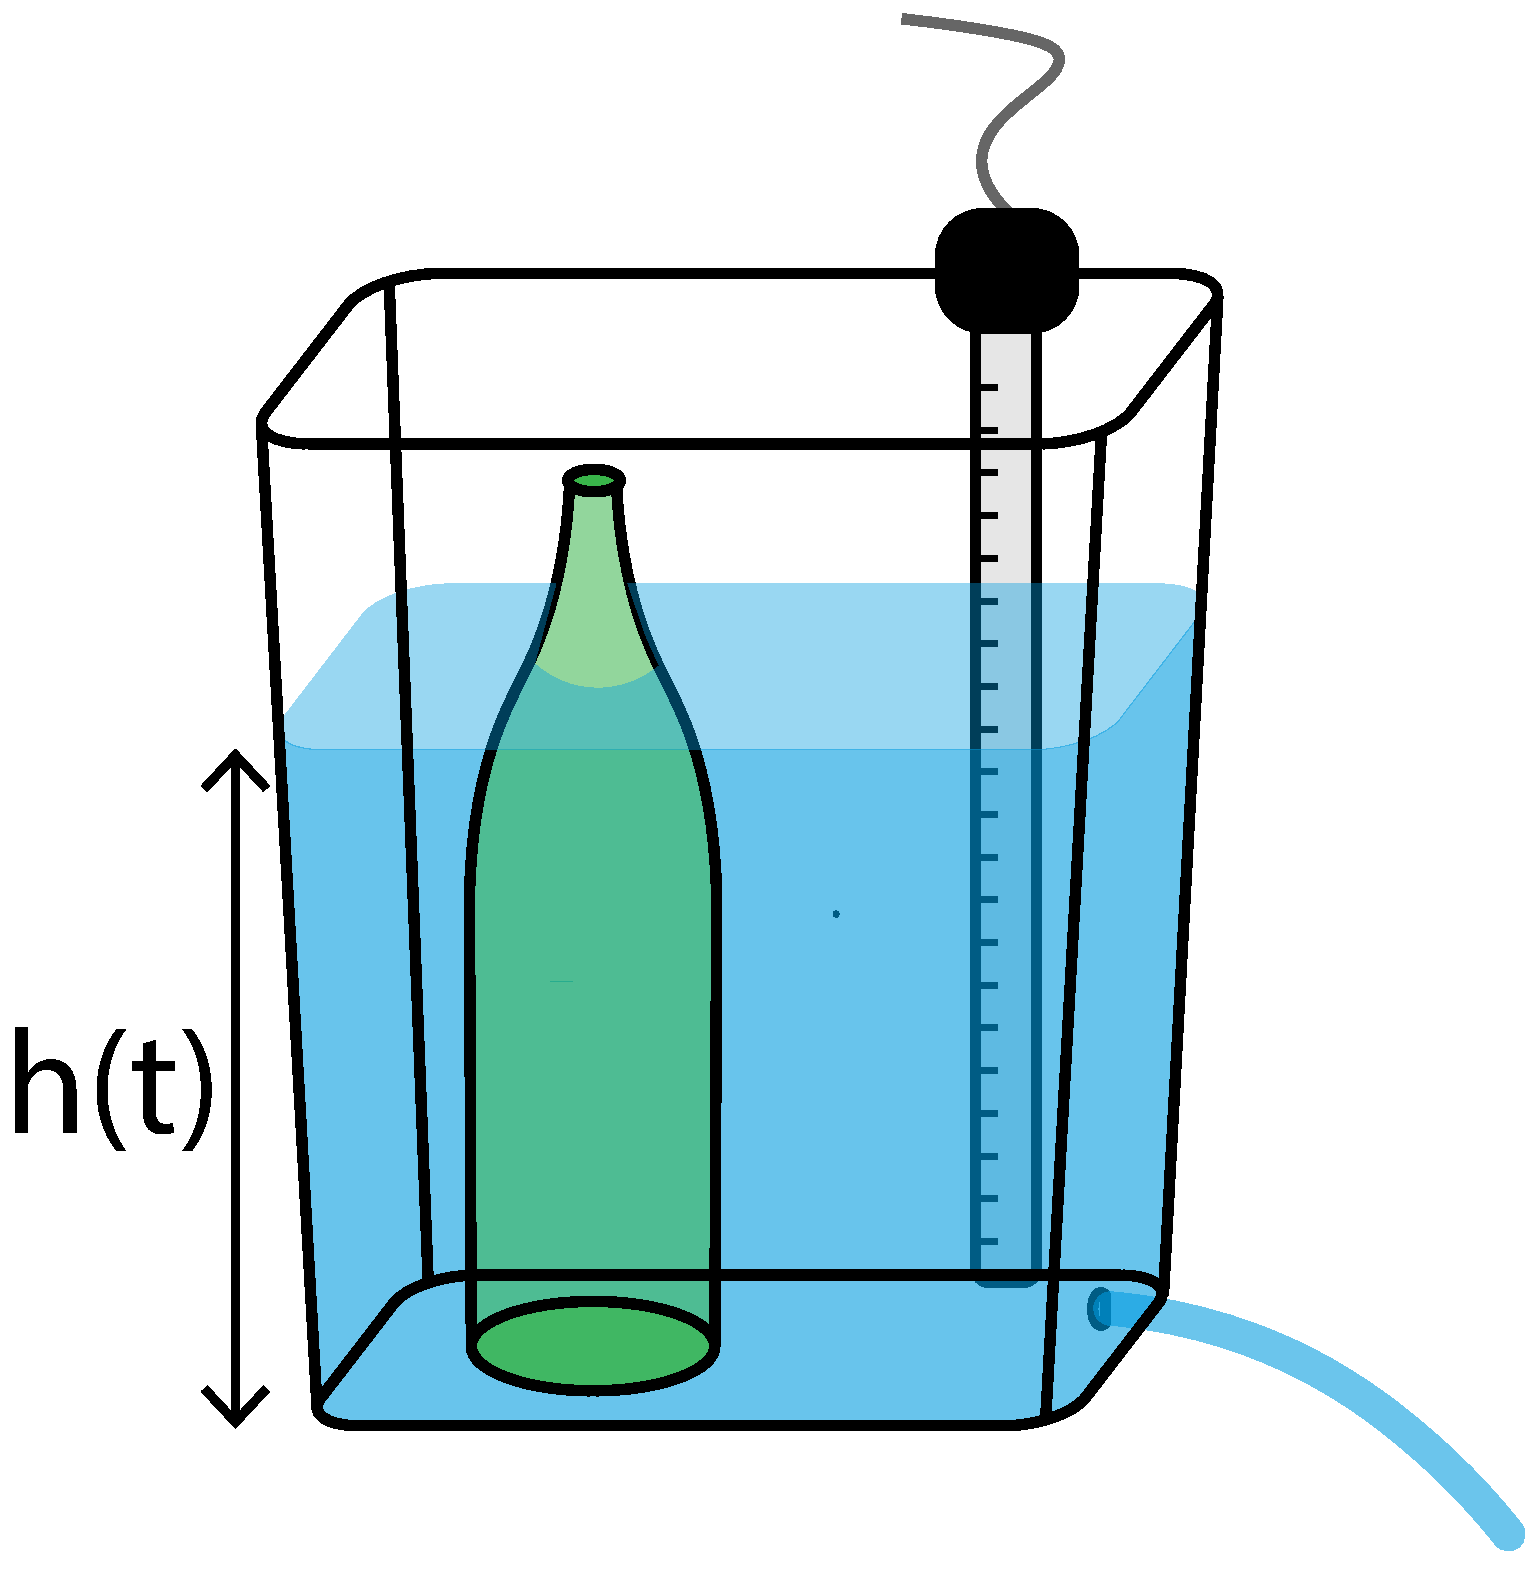
\includegraphics[height=0.375\textwidth]{../tank_geometry/tank_w_bottle.pdf}
	\includegraphics[height=0.375\textwidth]{../toy_h_w_object.pdf}
\end{center}

\absbreak % unclear why this is needed


\end{abstract}
%%%%%%%%%%%%%%%%%%%%%%%%%%%



\rsbreak

%%%%%%%%%% Insert the texts which can accomdate on firstpage in the tag "fmtext" %%%%%

\section{Introduction}
Throughout engineering and the applied sciences, we may encounter an open-top tank, draining of liquid via gravity-driven flow through a small orifice (a \emph{draining tank}).
Mathematical models of the dynamics of the liquid level in a draining tank are useful for designing the tank and orifice geometry, predicting emptying times, forecasting outlet flow rates, controlling the liquid level by manipulating an input stream, and inferring the liquid level from the outlet flow rate \cite{d2021torricelli,seborg2016process,groetsch1993inverse,groetsch1999inverse}.

\begin{mytcbox}[label=box:waterclocks, breakable]{Ancient water clocks}
Interestingly, ancient societies (e.g. ancient Greece) exploited the empirically predictable dynamics of the water level in a draining tank to measure and display the passage of time.
Specifically, the outflow \emph{clepsydra}, Greek for ``water thief'', was an open-top container with a small hole near its bottom and graduated markings on the inside. 
Filled with water then allowed to drain, the elapsed time was indicated by the liquid level with respect to the markings on the inside. \cite{bedini1962compartmented,hwang2021historical,ritner2016oriental,hejun1987research,schomberg2018karnak,mills1982newton}
The preserved Karnak clepsydra from $\sim$1300 BC \cite{schomberg2018karnak} is an inverted truncated cone. Notably, this geometry does not provide a constant rate of decrease in the water level; perhaps, though, its wider top was intended to compensate for faster outflow at higher water levels. An inverse problem pertaining to an outflow clepsydra is: what clepsydra shape provides a constant rate of decrease in the water level as it drains?
(Such a clepsydra may be obtained via a solid of revolution about the vertical axis such that the radius is proportional to the quartic root of the height. \cite{mills1982newton,d2021torricelli})
\end{mytcbox}
%Draining tanks have been studied since ancient times, as evidenced by water clocks in ancient Egypt, Greece, India, and China.
%The water clock, or clepsydra (Greek for ''water thief''), of the outflow design consisted of an open-top container, filled with water at some reference time, with a small orifice for outflow near its bottom.

%The geometry of an ideal clepsydra would produce a constant rate of decrease in the liquid level. However, the geometry of e.g. the preserved Karnak clepsydra from $\sim$1300 BC \cite{schomberg2018karnak}, an inverted truncated cone, does not. Though, perhaps, its wider top was intended to compensate for the faster outflow when the liquid level is higher.

% Italian physicist and mathematician 
Evangelista Torricelli (1608-1647) made a fundamental observation for mathematically modeling the liquid level in a draining tank: the velocity $v$ at which liquid flows out of a small orifice in a tank is proportional to the square root of the height of liquid above the orifice, $\Delta h$, i.e. $v\propto \sqrt{\Delta h}$ \cite{mills1982newton}.
% TODO: check that he didn't know g!
Today, we recover Torricelli's observation from Daniel Bernoulli's (1700–1782) equation \cite{welty2020fundamentals}, a mechanical energy balance applied to the steady, plug flow of an incompressible, inviscid fluid through the small orifice, neglecting frictional forces. This gives \emph{Torricelli's law}: $v=\sqrt{2 g \Delta h}$, with $g$ the acceleration due to gravity. \cite{d2021torricelli,teoman2022discharge}

A mass balance on a draining tank with Torricelli's law gives a first-order, [generally] nonlinear differential equation governing the liquid level in the tank over time \cite{groetsch1993inverse,seborg2016process,debook}.
The geometry of the tank affects the dynamics of the liquid level through its cross-sectional area as a function of height.
The cross-sectional area of the orifice affects the emptying time; theoretically, it gives the volumetric flow rate out of the tank from Torricelli's law. 
% TODO: a name for cross-sectional area parallel to the ground?
However, a \emph{discharge coefficient} \cite{de2000pin,blasone2015discharge,wadhwa2021study,liu2008drainage} must be introduced into the model for agreement with experimentally-measured volumetric outflow rates \cite{farmer1992physical,driver1998torricelli,brady2009siphons,rother2024modelling,paldy1963apparatus,ivanov2014testing,williams2021vessel,pavesi2019investigating,planinvsivc2011holes,saleta2005experimental,lopac2015water,powell2012carrying}.
The discharge coefficient \cite{teoman2022discharge,hicks2014determining,blasone2015discharge,lienhard1984velocity,wadhwa2021study}
(i) is defined as the ratio of the observed outlet volumetric flow rate to that predicted by Torricelli's law and the area of the orifice \cite{hicks2014determining};
(ii) accounts for (a) the vena contracta of the liquid jet (the cross-sectional area of the liquid jet issuing from the orifice is smaller than that of the orifice, owing to fluid streamlines in the tank, near the orifice, non-perpendicular to the orifice area \cite{horsch2020simple}), (b) frictional losses across the orifice, and (c) non-uniformity of the velocity profile; and
(iii) depends on the rheology of the liquid, the geometry of the orifice, and, for laminar flow, the Reynolds number \cite{teoman2022discharge}. 
%  and (ii) depends on the rheology of the fluid and the geometry of the orifice. 


In contrast to the \emph{forward problem} of using this dynamic model to predict the trajectory of the liquid level in a draining tank of a given geometry, Groetsch \cite{groetsch1993inverse,groetsch1999inverse} framed an \emph{inverse problem} \cite{groetsch1993inverse,neto2012introduction,tarantola2005inverse}: reconstruct the shape of the tank from its liquid level over time as it drains. 
While impossible to infer the precise geometry of the tank, one can leverage the dynamic model to determine the cross-sectional area of the tank as a function of height from the liquid level as a function of time. (The rate of decrease of the liquid level is indicative of the cross-sectional area of the tank at that height. The outlet flow rate depends on the water height only, not width; so, wider [say, cylindrical] tanks drain more slowly.)
However, this inverse problem of reconstruction is unstable: small errors in the measured liquid level can cause large errors in the estimated area of the tank. \cite{groetsch1993inverse}

\subsection{Our contribution}
Herein, we employ Bayesian statistical inversion \cite{calvetti2018inverse,waqar2023tutorial,kaipio2006statistical,dashti2013bayesian} to solve, with quantified uncertainty, an inverse problem of reconstruction: infer the shape of an exogenous, heavy solid (of unknown geometry but incapable of holding water) contained in a draining tank (of known geometry) from measurements of the liquid level in the draining tank over time.
(Because the solid displaces liquid in the tank, the rate of decrease of the liquid level provides information about the cross-sectional area of the solid at the height of the liquid.
As the tank drains, the liquid ``scans'' the area of the solid as a function of height.)
To test our ability to reconstruct the shape of the solid in the tank, we conduct tank drainage experiments with water and collect water level time series data with a level sensing strip. First, we build and calibrate (i.e., determine the posterior distribution of the parameters of) (i) a forward model of the dynamics of the water level in our draining tank and (ii) a probabilistic model of measurement noise from our level sensor.
For this task, we take length-measurements of the tank and orifice geometry and collect water level time series data from a tank drainage experiment without an exogenous solid. 
Second, we conduct a tank drainage experiment with an exogenous solid in the tank (a bottle). We then leverage this water level time series data and our calibrated forward and measurement models to obtain a posterior distribution over the area of the solid in the tank as a function of height.
Comparing with our [more] direct (via a tape measure) measurements of the solid's geometry, the inferred area of the solid traces its shape reasonably well ($\sim$10\% mean reconstruction error on the bottle's radius). 

%
%Because this reconstruction problem is unstable \cite{groetsch1993inverse}, 
%We employ Bayesian statistical inversion \cite{calvetti2018inverse,waqar2023tutorial,kaipio2006statistical,dashti2013bayesian} to predict the object's area as a function of height \emph{with quantified uncertainty}.

%To demonstrate and test our ability to solve this reconstruction problem, we conduct tank drainage experiments to collect liquid level time series data.
%We drilled a small hole in the side of an open-top tank, near the bottom.
%For each experiment, we fill the tank (perhaps, containing an exogenous heavy, solid object) with water, then allow it to drain (driven by gravity). A liquid level sensor, communicating with an Arduino microcontroller, measures the liquid level over time, giving liquid level time series data. 


%In this Bayesian approach, we treat each parameter/input in the problem as a random variable and model its probability distribution.
%The prior distribution expresses our beliefs and information about the parameters/inputs \emph{before} liquid level time series data are collected.
%After a tank drainage experiment, we use (a) the [forward] dynamic model of the liquid level, (b) a probabilistic model of the noise in the measured liquid level, and (c) liquid level time series data to construct the likelihood function, which expresses the support the data lend for each possible parameter/input.
%Via Bayes's theorem, the posterior distribution of the parameters/inputs---conditioned upon the liquid level time series data---follows from the prior and likelihood. The posterior, the solution to the reconstruction problem, expresses a probability distribution over the object's cross-sectional area as a function of height, in light of the the liquid level time series data from a drainage experiment.

% The structure of our paper is as follows. Sec.~\ref{sec:expt} describes our setup for tank drainage experiments.
\section{Setup for tank drainage experiments} \label{sec:expt}
First, we describe our experimental setup in Fig.~\ref{fig:photo_of_tank} for tank drainage (of water) experiments.

We possess a plastic, open-top tank---an inverted, right, truncated cone with a rounded rectangle base. 
The cross-sectional area [parallel to the ground] of the tank as a function of height $h$ [cm] from its bottom base is:
\begin{equation}
	a(h) = \frac{h}{h_{\text{max}}}a_t + \left(1-\frac{h}{h_{\text{max}}}\right) a_b, \label{eq:a_of_h}
\end{equation}
with $h_{\text{max}}$ [cm] the height of the tank and $a_b$ and $a_t$ [cm$^2$] the area of the rounded rectangle forming the bottom and top, respectively, base of the tank.
We drilled a small, circular orifice of radius $r_o$ [cm] in the side of the tank, parallel with the ground and a small height $h_o$ [cm] (to its center) from the bottom base.

A tank draining experiment constitutes: 
(1) optionally, placing an exogenous, heavy solid inside the tank; 
(2) filling the tank with water, to an initial height $h_0$ [cm]; 
(3) at time $t=0$ [s], allowing the water to drain out (driven by gravity) through the orifice; and 
(4) collecting time series data of the water level in the tank over time, $\{(t_i, h_{\text{obs}, i}) \}$, from a liquid level sensor communicating with an Arduino microcontroller. 

The exogenous [rigid] solid (i) is heavier than water, and thus remains stationary at the bottom of the tank; (ii) displaces water in the tank; and (iii) has a geometry rendering it incapable of holding water\footnote{A solid cannot hold water iff it is locally convex at points on its (assume, smooth) surface where the normal vector to the surface is anti-parallel with the gravitational field.}. 
Let $\alpha(h)$ [cm$^2$] be the cross-sectional area of this solid as a function of height $h$.

\begin{figure}[h!]
\begin{center}
	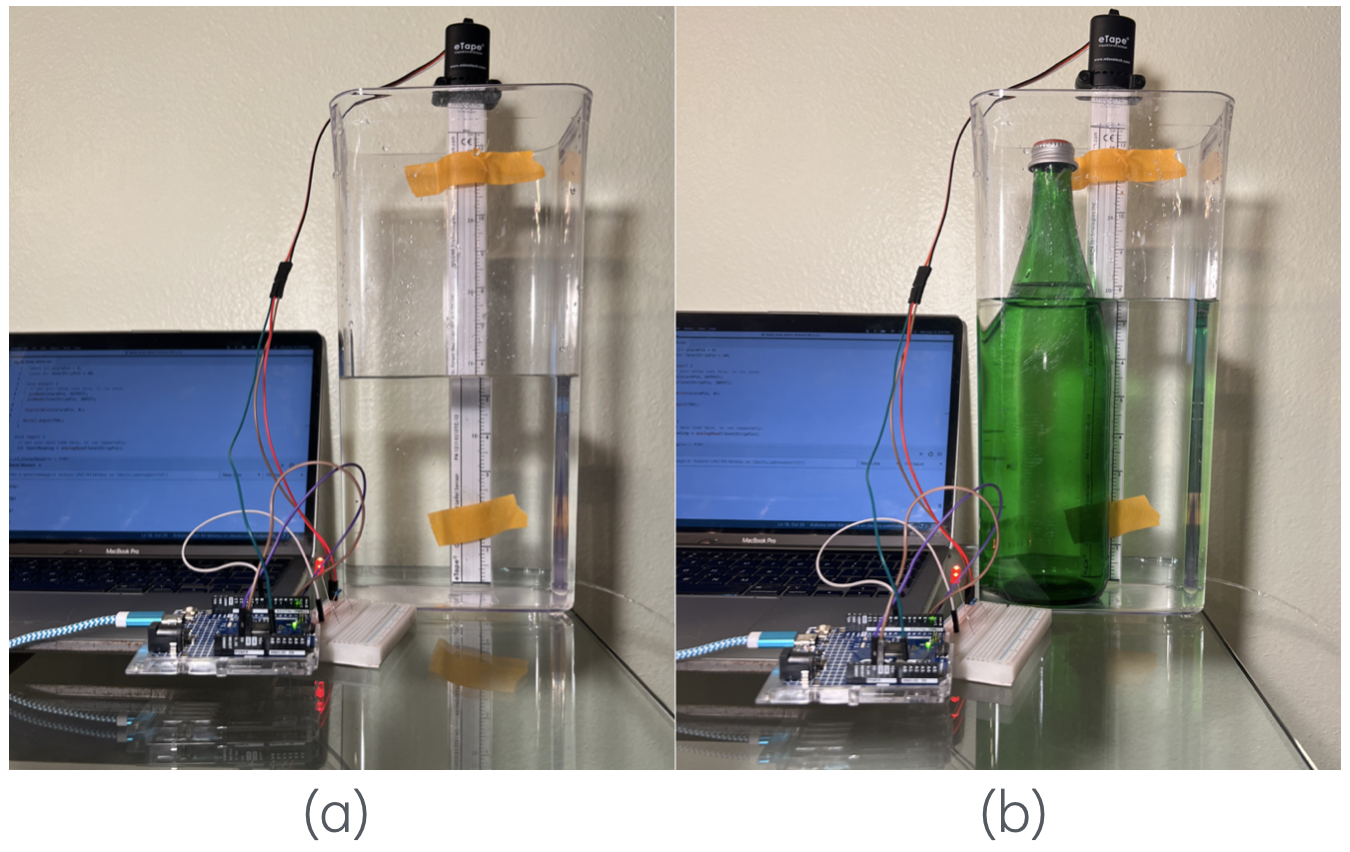
\includegraphics[width=0.65\textwidth]{../real_expt/real_expt.png}
	\caption{\textbf{Setup for tank drainage experiments} for (a) model calibration and (b) shape reconstruction.
	We fill our open-top tank (perhaps, containing an exogenous solid) with water, then allow it to drain via gravity-driven flow out of a small hole in its side, near its bottom. A liquid level strip measures the water level in the tank over time, giving time series data.
	}
	\label{fig:photo_of_tank}
\end{center}
\end{figure}

\paragraph{The liquid level sensor.}
We place an eTape\texttrademark\xspace liquid level strip vertically inside the tank, immersed in the water. 
The level strip gives an electrically-resistive output inversely proportional to the water level owing to its compression by the hydrostatic pressure of the water in which it is immersed \cite{eTape}.
The sensor communicates with an Arduino microcontroller, providing us measurements of the water level over a sequence of times. 
To map the reading from the level sensor [0-1023 integer values] to the liquid level in the tank [cm], we constructed a calibration curve (a smooth 1D spline) with a resolution of 1 cm.

\section{The forward and measurement models and likelihood} \label{sec:forward_model}
The [deterministic] \emph{forward model} predicts the water level $h(t)$ [m] in our draining tank over time $t$ [s], given the \emph{inputs} $\alpha(h)$ and $h_0$ and \emph{parameters} $a_t$, $a_b$, $h_{\text{max}}$, $r_o$, $h_o$, and the discharge coefficient $c$. 
The probabilistic \emph{measurement model} characterizes the noise contaminating a water level measurement $h_{\text{obs}}$ made by our sensor.
After we collect time series data \thedata from a tank drainage experiment, we use the forward and measurement models to construct the \emph{likelihood function}---the probability density of the data \thedata conditioned upon proposed functions/values for the inputs/parameters. 
When any of the inputs/parameters are uncertain in an inverse problem concerning the draining tank, the likelihood function quantifies the support that the data \thedata lend for each possible set of inputs/parameters.

\subsection{Forward model}
Here, we mathematically model the height of water in our draining tank as a function of time, $h(t)$. (We assume the water at the top of the tank remains flat---allowed by a slow outflow rate). 
%We treat the water as incompressible (constant density: $\rho$ [g/cm$^3$]) and inviscid. 
%Our model follows from (i) the law of conservation of mass and (ii) Torricelli's law.
% outflow driven by gravity exerting a force on the water above the orifice, causing a hydrostatic pressure in the water at the entrance of the orifice. 

\paragraph{Torricelli's law.}
We model the velocity $v$ [cm/s] of the jet of water flowing out of the orifice at time $t$, when the water height is $h(t)$, with Torricelli's law \cite{d2021torricelli}:
\begin{equation}
	v(h(t)) =  \sqrt{2 g(h(t)-h_o)}, \label{eq:Torricelli}
\end{equation} where $g$ [cm/s$^2$] is the acceleration due to gravity. Torricelli's law follows from Bernoulli's equation \cite{welty2020fundamentals}, a mechanical energy balance on the flow through the orifice, treating (i) the flow as steady, plug, and absent of frictional forces and (ii) the water as inviscid and incompressible.
Torricelli's law matches (i) the gain in kinetic energy, $(\Delta m) v^2/2$, when a small mass $\Delta m$ of water is ejected from the orifice, with (ii) the loss of gravitational potential energy, $(\Delta m)g(h-h_o)$, from the concomitant removal of a small slice of water of mass $\Delta m$ from the top of the body of water in the tank. \cite{groetsch1993inverse,driver1998torricelli,williams2021vessel}

\paragraph{Volumetric outflow rate.}
%If Torricelli's law held and the cross-sectional area of the liquid jet out of the tank were the same as the cross-sectional area of the orifice ($\pi r_o^2$), the volumetric flow rate out of the tank would be $v\pi r_o^2$.
Invoking Torricelli's law, we model the volumetric flow rate out of the tank at time $t$, when the water height is $h(t)$, as:
\begin{equation}
	c \pi r_o^2 \sqrt{2 g(h(t)-h_o)}, \label{eq:outletflow}
\end{equation}
with $c\in(0,1)$ the [dimensionless] discharge coefficient---a ``fudge factor'' to account for the vena contracta in the water jet, non-plug flow through the orifice, and frictional losses as the water flows through the orifice \cite{horsch2020simple,teoman2022discharge,hicks2014determining,blasone2015discharge,lienhard1984velocity,wadhwa2021study}. 
Note, $c=1$ corresponds with an ideal water jet with cross-sectional area equal to that of the orifice ($\pi r_o^2$), plug flow, and zero frictional losses.

\paragraph{Volume of water in the tank.} 
The volume $V$ [cm$^3$] of water in the tank at time $t$, when the water height is $h(t)$, follows from the method of cross-sections in calculus \cite{debook}:
\begin{equation}
	V(h(t))=\int_0^{h(t)} \left[a(y) - \alpha(y) \right] dy. \label{eq:volume}
\end{equation}
The integrand is the cross-sectional area of water in the tank at height $y$; subtraction of the area of the solid $\alpha(y)$ from the area of the tank $a(h)$ accounts for the solid displacing water. (We neglect the small volume of water displaced by the level sensor.) The expression assumes the solid did not retain water above $h(t)$.

\paragraph{Conservation of mass.}
% A mass balance on the draining tank [as the control volume] at time $t \geq 0$ equates the rate of decrease of water in the tank [g/s] with the outflow rate [g/s].
Treating the water as incompressible (constant density: $\rho$ [g/cm$^3$]) and using expression~\ref{eq:outletflow} for the outflow, a mass balance on the draining tank for $t\geq 0$ gives:
\begin{equation}
	\overbrace{\diff{}{t} \Bigl( \rho V(h(t)) \Bigr )}^{\text{rate of accumulation}}= - \overbrace{\rho c \pi r_o^2 \sqrt{2 g(h(t)-h_o)}}^{\text{rate of outflow}}. \label{eq:massbalance}
\end{equation}
Differentiating $V(h(t))$ in eqn.~\ref{eq:volume} and using the chain rule \cite{debook} to rewrite the accumulation term gives our forward model for $h(t)$:
%\begin{empheq}[box=\mybox]{align}
\begin{empheq}[box={\Garybox[forward model]}]{align}
& \left[ a(h)-\alpha(h)\right] \diff{h}{t}= -c \pi r_o^2 \sqrt{2g (h(t)-h_o)}, \,\,\, t \geq 0 \label{eq:forward_model} \\
& h(0)=h_0, \nonumber
\end{empheq}
a [generally] nonlinear, first-order, ordinary differential equation (ODE) in $h(t)$ subject to an initial condition.
Given the geometry of the tank and solid through $a(h)$ and $\alpha(h)$, the discharge coefficient $c$, the orifice radius and height $r_o$ and $h_o$, and initial water height $h_0$, we numerically solve the ODE in eqn.~\ref{eq:forward_model} (with \texttt{DifferentialEquations.jl} \cite{rackauckas2017differentialequations}, which uses a Runge-Kutta method \cite{tsitouras2011runge}) to predict the water height in our draining tank over time, $h(t)$. 
% I.e., this \emph{forward} model makes predictions of the system output $h(t)$ (an \emph{effect}) when given the parameters and initial condition (the \emph{cause} of the effect).

\vspace{-\baselineskip}
\subparagraph{A regime of model invalidity.} If the radius of the orifice $r_o$ is small, surface tension of the water may stop flow out of the orifice when $h- h_o$ is positive (but small). In this regime, Torricelli's law and thus our forward model do not hold.

\vspace{-\baselineskip}
\subparagraph{Parameterizing the object's area as a function of height.}
We parameterize the area of the solid inside the tank as a function of height, $\alpha(h)$, with a list of $n+1$ discrete evaluations of $\alpha(h)$ on a uniform grid of points on its domain $[0, h_{\text{max}}]$:
\begin{equation}
	\boldsymbol \alpha := [\alpha_0, \alpha_1, ... \alpha_n] \label{eq:alpha}
\end{equation}
where $\alpha_i :=\alpha(i \Delta h)$ for $i \in \{0, ..., n\}$, $\Delta h = h_{\text{max}}/n$, and $0 \leq \alpha_i \leq a(i\Delta h)$ for the solid to fit in the tank.
Then, we construct the function $\alpha(h)$ for $h\in [0, h_{\text{max}}]$ via piecewise, monotonic, cubic interpolation \cite{fritsch1984method} of the function values in $\boldsymbol \alpha$. (\emph{Monotonic} interpolation prevents the unphysical outcome of $\alpha(h) > a(h)$ for any $h \in [0, h_{\text{max}}]$.) 
%From another perspective, we express the solid's area as a function of height as:
%\begin{equation}
%	\alpha(h; \boldsymbol \alpha) = \sum_{i=0}^n \alpha_i \phi(h-i \Delta h) \label{eq:alpha_basis}
%\end{equation} where $\phi(x)= \max(0, 1-\lvert x \rvert / (\Delta h)) $ is a triangle ``tent'' basis function \cite{hat_functions}.

\vspace{-\baselineskip}
\subparagraph{Inputs, output, and model parameters.} 
We
%In the language of inverse problems \cite{groetsch1999inverse,waqar2023tutorial}, we 
consider the solid's area $\boldsymbol \alpha$ and initial water level $h_0$ as \emph{inputs} (causal factors) to the system and the water level as a function of time $h(t)$ as the \emph{output} (effect) of the system.
The \emph{model parameters} $\boldsymbol \theta \in \mathbb{R}^6$ characterize the geometry of the tank and orifice and, loosely, the rheology of water (embedded in $c$):
\begin{equation}
	\boldsymbol \theta := [h_{\text{max}}, a_b, a_t, r_o, h_o, c]. \label{eq:theta}
\end{equation}
(We omit $g$ from $\boldsymbol \theta$ because we treat it as a constant known with certainty.)
Hereafter, we write the forward model as \themodel to indicate the dependence of $h(t)$ on the inputs and parameters.

\subsection{Measurement model}
Suppose at time $t$ our water level sensor measures the height of water in the tank, providing a data point $(t, h_{\text{obs}})$ (obs for ``observation''). 
To model [unobservable] noise corrupting the measurement, we treat the measured water level $h_{\text{obs}}$ as a realization of a random variable
\begin{equation}
	H_{\text{obs}} = \themodelnomath + \Psi,
\end{equation}
with the Gaussian-distributed random variable $\Psi \overset{\text{iid}}{\sim} \mathcal{N}(0, \sigma^2)$ the noise, additive to the model output and, among multiple measurements, independent and identically-distributed (iid). 
Then, the probability density of the measured liquid level is a Gaussian centered at the model prediction:
\begin{equation}
	H_{\text{obs}} \mid h_0, \boldsymbol \alpha, \boldsymbol  \theta, \sigma^2 \overset{\text{iid}}{\sim} \mathcal{N}(\themodelnomath, \sigma^2). \label{eq:H_obs_distn}
\end{equation} We are explicit that $H_{\text{obs}}$ is conditioned upon the inputs, parameters, and noise variance.
% Sources of this noise are: imprecision of the liquid level strip, our calibration curve for the liquid level strip, vibrations

% TODO: plot residuals
% TODO expand 

\subsection{Likelihood function}
The likelihood is the $N$-dimensional probability density of observing $\mathbf{h}_\text{obs}:=(h_{\text{obs},1}, ..., h_{\text{obs},N})$ in time series data \thedata (with each measurement time $t_i$ set) given the inputs $h_0$ and $\boldsymbol \alpha$, model parameters $\boldsymbol \theta$, and noise variance $\sigma^2$. 
Based on eqn.~\ref{eq:H_obs_distn}, the likelihood density is:
\begin{equation}
 \pi_{\text{like}}(\thedatanomath \mid h_0,\boldsymbol  \alpha, \boldsymbol \theta, \sigma^2 ) = \prod_{i=1}^N \frac{1}{\sqrt{2\pi\sigma^2}} \exp \left[-\frac{1}{2}\left(\frac{h_{\text{obs}, i} - h(t_i; h_0, \boldsymbol\alpha, \boldsymbol\theta)}{\sigma} \right)^2 \right]. \label{eq:like}
\end{equation}
Once we obtain the data \thedata, we view the likelihood as a function of $h_0$, $\boldsymbol \alpha$, $\boldsymbol \theta$, and $\sigma^2$.
The likelihood function (i) scores the consistency between (a) the model predictions of the water level over time, with proposed values for the inputs and parameters, and (b) the water level time series data and, hence, (ii) quantifies the support the data lend for each possible set of values for the inputs and parameters \cite{van2021bayesian}. 
% The key idea is: if the data were likely (unlikely) to be obtained under proposed values for the inputs and parameters, then the 

\section{Bayesian statistical inversion (BSI)} \label{sec:bsi}
Here, we outline Bayesian statistical inversion (BSI)  \cite{calvetti2018inverse,waqar2023tutorial,kaipio2006statistical,dashti2013bayesian,allmaras2013estimating}, a tool for solving inverse problems while incorporating prior information and quantifying uncertainty. 
Later, we employ BSI to, using water level time series data from tank drainage experiments,  
(1, parameter inference) calibrate our forward and measurement models and 
(2, reconstruction) infer the shape of a solid in the tank.

Under BSI, we treat the uncertain input(s) and/or parameters of a tank drainage experiment as random variables and model their probability distributions.
The probability density over input/parameter space expresses our knowledge and beliefs about the inputs/parameters, namely 
(i) they most likely lie in the region containing the bulk of the density and (ii) the spread (concentration) of the density quantifies our uncertainty (certainty) about them. 

%A may summarize the state of our knowledge and beliefs about an input/parameter through the moments of its probability distribution (e.g., mean and variance) with the other inputs/parameters marginalized out. 

The BSI approach to inverse problems with draining tanks follows three stages:

\vspace{-\baselineskip}
\paragraph{(1) specify the prior.}
Before we allow the tank to drain and observe water level time series data, we express our knowledge and [to an extent, subjective] beliefs about the inputs and parameters through a \emph{prior} probability density $\pi_{\text{pr}}(h_0, \boldsymbol \alpha, \boldsymbol \theta, \sigma^2)$.
The [marginal] prior density on an input/parameter can range from 
(i) diffuse (eg.\ a uniform distribution) if we lack knowledge about it, adopting the principle of indifference, to 
(ii) informative (eg.\ a Gaussian with a small variance) if we possess a [noisy] measurement of it. 
\cite{van2021bayesian}

\vspace{-\baselineskip}
\paragraph{(2) gather data and construct the likelihood.}
Next, we conduct a tank drainage experiment (perhaps, containing an exogenous solid) to collect water level time series data, \thedata. 
When considered against the forward and measurement models, these data provide new information about the inputs and parameters. The likelihood function $\pi_{\text{like}}(\thedatanomath \mid h_0,\boldsymbol  \alpha, \boldsymbol \theta, \sigma^2 )$ quantifies the support the data lend for different inputs and parameters.

\vspace{-\baselineskip}
\paragraph{(3) update the prior to a posterior.}
In light of the data \thedata, we invoke Bayes's theorem  \cite{van2021bayesian,calvetti2018inverse} to update our prior density of the inputs and parameters to a \emph{posterior} density
\begin{equation}
	\pi_{\text{post}}(h_0, \boldsymbol \alpha, \boldsymbol \theta, \sigma^2 \mid \thedatanomath) \propto % \frac{
	\pi_{\text{like}}(\thedatanomath \mid h_0,  \boldsymbol \alpha, \boldsymbol \theta, \sigma^2 ) 
	\pi_{\text{pr}}(h_0, \boldsymbol\alpha, \boldsymbol \theta, \sigma^2).
	%}{
	%\pi_{\text{ev}}(\thedatanomath) 
	%},
	 \label{eq:post}
\end{equation} 
A compromise between the likelihood and prior,
the posterior density expresses our knowledge and beliefs about the inputs and parameters \emph{conditioned upon the data} [and, implicitly, the structure of our forward and measurement models]. 
Thus, the posterior represents the raw, uncertainty-quantifying solution to the inverse problem.
Note, uncertainty (entropy) remains in the posterior because
 (i) our measurements are noisy and 
 (ii) perhaps, even noiseless data cannot fully constrain a subset of the parameters/inputs.
(The normalizing factor for the posterior, the \emph{evidence}, is a high-dimensional integral that can, in principle, be computed from the likelihood and prior.)


%The posterior may be 
%(i) summarized with a \emph{credible region} [that contains the bulk of the posterior density] for each parameter/input;
%(ii) queried e.g., ``what is the probability this input/parameter exceeds a certain value?''; and
%(iii) exploited in conjunction with the forward model to make probabilistic predictions, such as predicting the distribution of emptying times for a draining tank.

\vspace{-\baselineskip}
\subparagraph{Sampling from the posterior distribution.} 
We conduct Markov chain Monte Carlo (MCMC) simulations \cite{robert1999monte,van2021bayesian} to sample inputs/parameters $(h_0, \boldsymbol \alpha, \boldsymbol \theta, \sigma^2 )$ from the posterior density $\pi_{\text{post}}(h_0, \boldsymbol \alpha, \boldsymbol \theta, \sigma^2 \mid \thedatanomath)$. 
From samples \thesamples from the posterior, we may draw empirical posterior distributions, compute credible intervals, and plot samples of liquid level trajectories when paired with the forward model.
Specifically, we use the No-U-Turn Sampler (NUTS) \cite{hoffman2014no} implemented in the probabilistic programming language \cite{gordon2014probabilistic} \texttt{Turing.jl} \cite{ge2018turing}.
A key advantage of MCMC samplers is that we can circumvent computing the evidence. 


\section{Results}
We now employ BSI to, using water level time series data from tank drainage experiments,  
(1, parameter inference) calibrate our forward and measurement models then
(2, reconstruction) exploit our calibrated model to infer the shape of a solid contained in the tank.

\subsection{Phase I: Bayesian calibration of the forward and measurement models}
\label{sec:phaseI}
Our objective now is to calibrate then test our forward and measurement models.
At this point, the model parameters $\boldsymbol \Theta$ and measurement noise variance $\Sigma^2$ are highly uncertain.
To gather information about $\boldsymbol \Theta$ and $\Sigma^2$, we (a) take length-measurements of the tank and orifice geometry and (b) collect water level time series data from a tank drainage experiment devoid of a solid (certainly, $\boldsymbol \alpha = \mathbf{0}$).
The \emph{calibrated model} constitutes eqns.~\ref{eq:forward_model} and \ref{eq:H_obs_distn} with the resulting posterior distribution of $\boldsymbol \Theta$ and $\Sigma^2$. We test the calibrated model for its capability to predict the liquid level trajectory in a replicate tank drainage experiment.

% The key idea is that our length-measurements of the tank and orifice geometry and water level time series data from a drainage experiment in a tank without an object provide information about the parameters and measurement noise variance. 
%Hopefully, the calibrated model will allow us to accuracy solve the reconstruction problem in Phase II. 
% Here, we also conduct a replicate experiment for testing the calibrated model. 
% Since we directly measured the other parameters in $\theta$, the two primary unknowns for our model calibration phase are the discharge coefficient $C$ and noise variance $\Sigma^2$. 

\subsubsection{Experimental setup}
We set up a tank draining experiment with an initial water level (measured by the level strip) $h_{0, \text{obs}}=26.54$\,cm. 
With certainty, the tank does not contain an exogenous solid. See Fig.~\ref{fig:naked_tank}.

\subsubsection{Prior distributions} 
We express our knowledge and beliefs about the inputs and parameters, before allowing the tank to drain and observing water level time series data, by constructing a prior density $\pi_{\text{pr}}(h_0, \boldsymbol \alpha, \boldsymbol \theta, \sigma^2)$ variable-by-variable (assuming independence). 
\vspace{-\baselineskip}
\subparagraph{Tank geometry.} We use a measuring tape to make length-measurements of the dimensions of the tank.
Specifically, we measure the length, width, and perimeter of the rounded rectangle forming the top and bottom of the tank,
$l_{t, \text{obs}}=14.6$\,cm, $w_{t, \text{obs}}=9.0$\,cm, $p_{t, \text{obs}}=44.3$\,cm,
$l_{b, \text{obs}}=13.4$\,cm, $w_{b, \text{obs}}=7.8$\,cm, and $p_{b, \text{obs}}=40.1$\,cm, and the height of the tank $h_{\text{max}, \text{obs}}=28.6$\,cm.
Informed by these [noisy and imprecise] measurements, we impose Gaussian prior distributions:
\begin{align}
L_{t,b} &\sim \mathcal{N}(l_{t,b, \text{obs}}, \sigma_\ell^2) \\
W_{t,b} &\sim \mathcal{N}(w_{t,b, \text{obs}}, \sigma_\ell^2) \\
P_{t,b} &\sim \mathcal{N}(p_{t,b, \text{obs}}, \sigma_\ell^2) \\
H_{\text{max}} &\sim \mathcal{N}(h_{\text{max}, \text{obs}}, \sigma_\ell^2)
\end{align}
where $\sigma_\ell=0.1$\,cm is the [assumed] standard deviation of our length-measurements, based on the markings on our measurement tape. 
For the area of the rounded rectangle forming the top and bottom of the tank,
we (i) solve for the radius of the circles at the four corners $R_{t/b}$ consistent with these measurements using $P_{t,b}=2(\pi R_{t,b} + L_{t,b}+W_{t,b}-4R_{t,b})$ then (ii) compute the area \cite{rounded_rect}
\begin{equation}
	A_{t,b}= (L_{t,b}-2R_{t,b})(W_{t,b}-2R_{t,b})+ 2R_{t,b} (L_{t,b}+W_{t,b} -4R_{t,b}) + \pi R_{t,b}^2.
\end{equation}
The prior distributions of $A_t$ and $A_b$ follow accordingly. 
(This gives point estimates $a_{t, \text{obs}}=129.9$\,cm and $a_{b, \text{obs}}=103.0$\,cm.)

\vspace{-\baselineskip}
\subparagraph{Orifice height and geometry.} 
We measure the height of the orifice in the side of the tank as $h_{o, \text{obs}}=0.9$\,cm and impose an informative prior:
\begin{equation}
H_o \sim \mathcal{N}(h_{o, \text{obs}}, \sigma_\ell^2).
\end{equation}
Informed by the manufacturer-reported diameter (5/64\,in) of the drill bit we used to drill the hole in the tank, we estimate the radius of the orifice as $r_{o, \text{obs}}=0.1$\,cm and impose the prior:
\begin{equation}
R_o \sim \mathcal{N}(r_{o, \text{obs}}, \sigma_d^2), \label{eq:R_o_prior}
\end{equation}
where $\sigma_d= 0.001$\,cm expresses uncertainty in the bit radius and its translation into an orifice.

\vspace{-\baselineskip}
\subparagraph{Exogenous solid geometry.}
With certainty, no solid resides in the tank, so $\boldsymbol \alpha=\mathbf{0}$. Technically, this is a Dirac delta prior density on $\mathbf{A}$, $\pi_{\text{pr}}(\boldsymbol \alpha)=\delta(\boldsymbol \alpha - \mathbf{0})$. 


% TODO mention truncations


\vspace{-\baselineskip}
\subparagraph{Discharge coefficient.} 
Our prior distribution on the discharge coefficient is weakly informed:
\begin{equation}
	C \sim \mathcal{N}(0.65, 0.25^2).
\end{equation} The mean is a reported discharge coefficient for water flow through a round orifice \cite{hicks2014determining}. 

\vspace{-\baselineskip}
\subparagraph{Variance of measurement noise.} 
We impose a uniform prior on the standard deviation of the noise emanating from our water level sensor:
\begin{equation}
\Sigma \sim \mathcal{U}(0\,\text{cm}, 0.5\,\text{cm}),
\end{equation} whose generous upper bound is informed by our experience in calibrating the liquid level strip. 

\vspace{-\baselineskip}
\subparagraph{Initial water level.} We impose an informative prior distribution on the initial water level based on the initial reading of the water level sensor:
\begin{equation}
	H_0 \mid \Sigma=\sigma \sim \mathcal{N}(h_{0, \text{obs}}, \sigma^2).
\end{equation} 

\paragraph{Visualization of the prior.}
Together with the forward model in eqn.~\ref{eq:forward_model}, $\pi_{\text{pr}}(h_0, \boldsymbol \alpha, \boldsymbol \theta, \sigma^2)$ gives a prior distribution over water level trajectories in the tank, \themodel. 
Fig~\ref{fig:prior_train} shows samples of functions \themodel from the prior, which encodes a broad range of possible future trajectories. 

\subsubsection{Water level time series data from a tank-drainage experiment} At time $t:=0$, we allow the tank to drain of water while our level sensor records the water level over time. 
Fig.~\ref{fig:posterior_train} shows the resulting water level time series data \thedata.

\subsubsection{Posterior distribution}
The posterior distribution $\pi_{\text{post}}(h_0, \boldsymbol \alpha, \boldsymbol \theta, \sigma^2 \mid \thedatanomath)$ follows from our prior and likelihood function constructed from the data \thedata (see eqn.~\ref{eq:post}). 
We employ NUTS to draw $N_s=1000$ samples \thesamples from the posterior over three independent chains, excluding the first half of each chain discarded for ``burn-in''. 
(We omit the last three data points because surface tension stopped flow out of the orifice despite $h>h_o$---unaccounted for in the model.)

%TODO how many samples

\paragraph{Visualization of the posterior.}Fig.~\ref{fig:posterior_train_theta} visualizes the empirical posterior distribution. 
The top panel shows the [marginal] empirical posterior distributions (histograms) of the parameters and initial water level along with their 80\% equal-tailed credible intervals. 
For the variables we measured with our measuring tape, the credible intervals are centered at the measurements. 
The measured initial water level, however, falls outside of the credible interval; a higher initial water level than measured is consistent with the time series data \thedata.
The bottom panel shows the covariance matrix of the parameters and input. Eg. $c$ positively covaries with both $a_t$ and $a_b$ because the dynamics of $h(t)$ depend on the ratio $c/a(h)$.

%The information that the data from this tank-draining experiment provided about $C$ and $\Sigma$ will be useful for the reconstruction inverse problem of inferring the shape of an object inside the tank from water level time series data. (We assume the object does not affect the discharge coefficient nor noise in the liquid level sensor.)

\paragraph{Posterior predictive check.} 
Water level trajectories \themodel, with $(\thevars)$ sampled from the posterior distribution, in Fig.~\ref{fig:posterior_train} agree reasonably with the measured water levels over time (mean absolute residual: 0.26\,cm). 
Comparing the prior and posterior distributions of water level trajectories in Fig.~\ref{fig:prior_train} and Fig.~\ref{fig:posterior_train}, the reduced variance in the trajectories reflects information about the parameter vector gained from considering the water level time series data against the forward and measurement models.

\begin{figure}[!ht]
    \centering
        \begin{subfigure}[b]{0.225\textwidth}
    	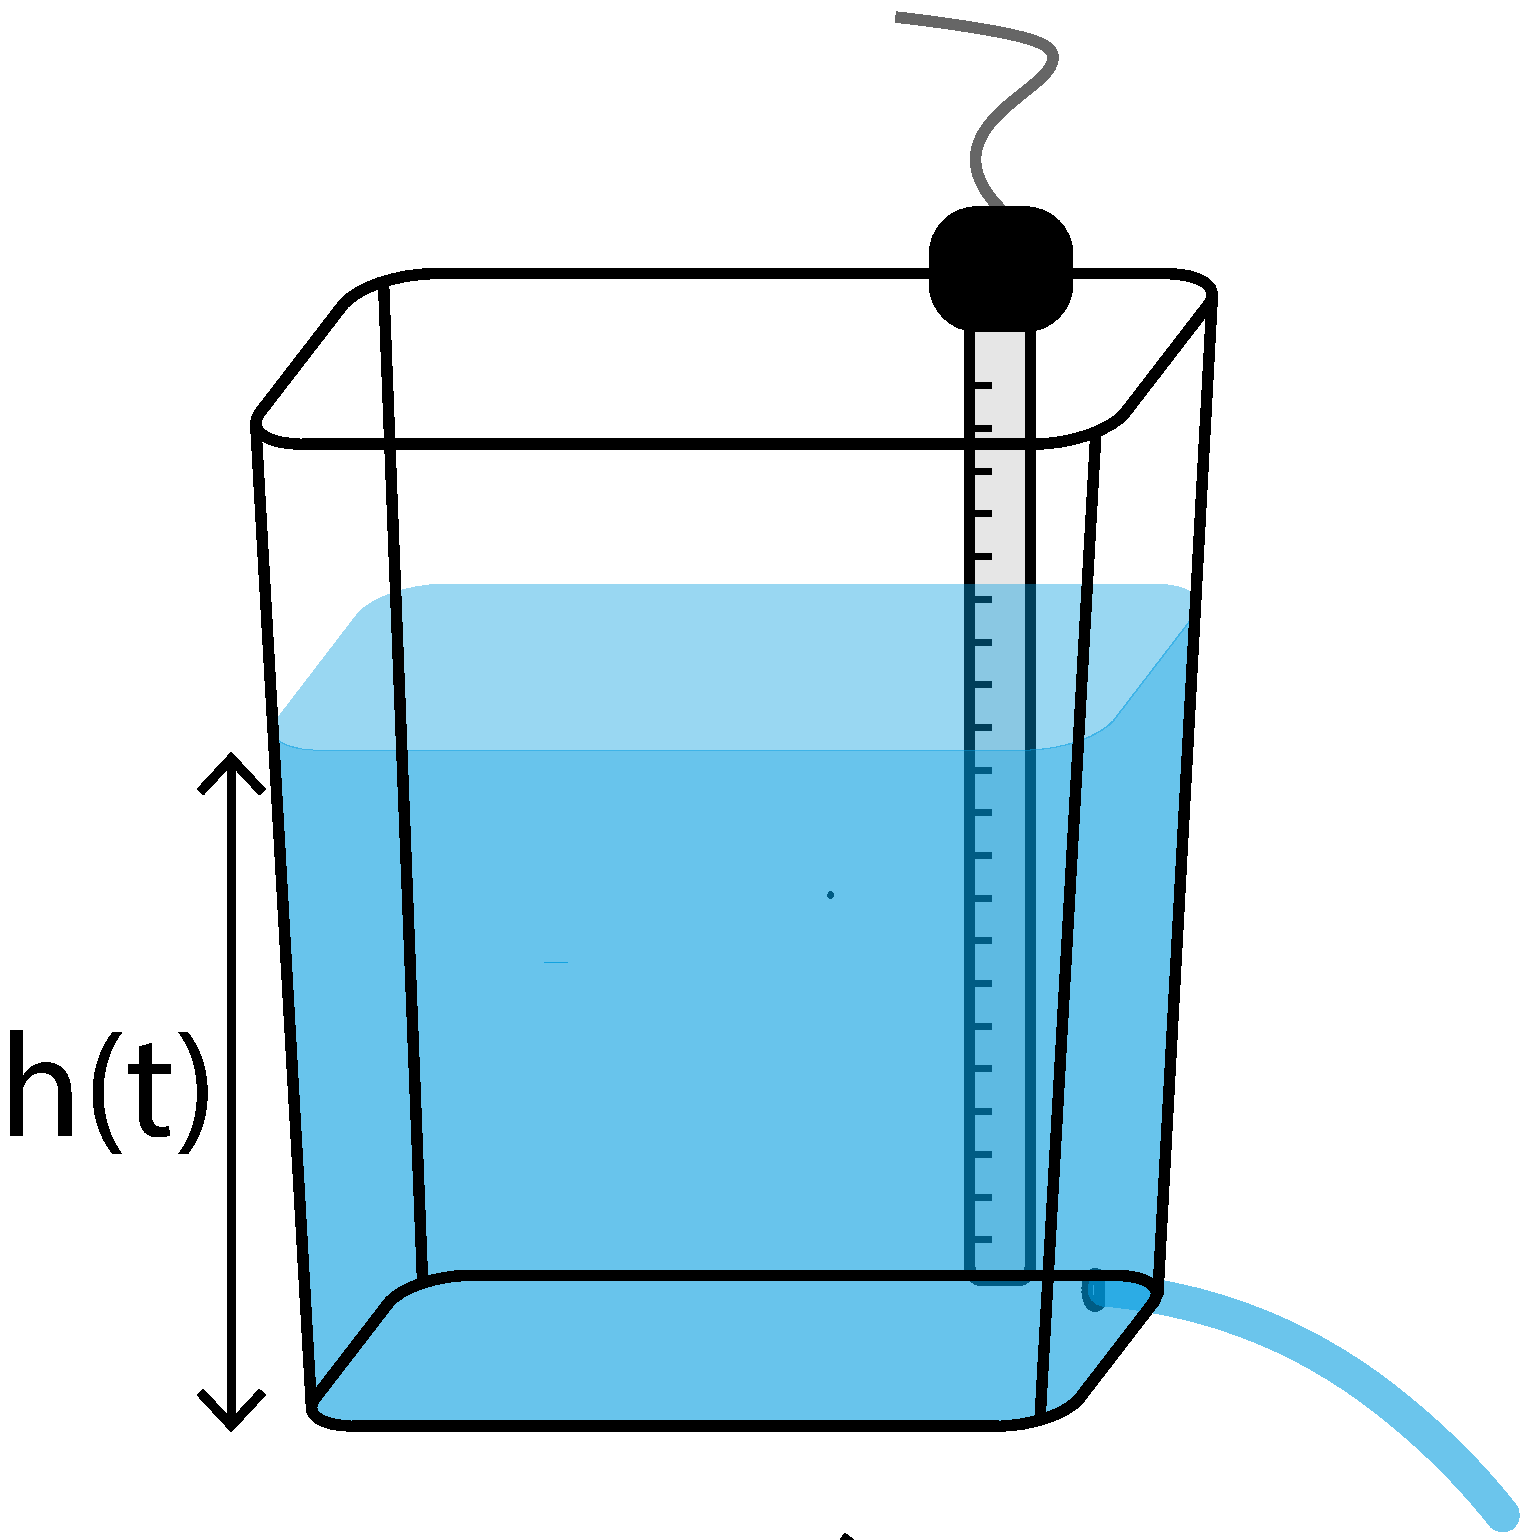
\includegraphics[width=\textwidth]{../tank_geometry/naked_tank.pdf}
	\caption{Experiment setup} \label{fig:naked_tank}
    \end{subfigure}
    
     \begin{subfigure}[b]{0.4\textwidth}
    	\includegraphics[width=\textwidth]{../prior_train.pdf}
	\caption{Prior distribution} \label{fig:prior_train}
    \end{subfigure}
     \begin{subfigure}[b]{0.4\textwidth}
    	\includegraphics[width=\textwidth]{../posterior_train.pdf}
	\caption{Data \& posterior distribution} \label{fig:posterior_train}
    \end{subfigure}
    
     \begin{subfigure}[b]{\textwidth}
     \center
    	\includegraphics[width=0.75\textwidth]{../posterior_train_theta.pdf}
	\includegraphics[width=0.375\textwidth]{../posterior_cov_matrix.pdf}
	\caption{Posterior distribution} \label{fig:posterior_train_theta}
    \end{subfigure}
    \caption{
      \textbf{Model calibration.}
      (a) We fill our tank (devoid of an exogenous solid) with water, then, at $t=0$, allow it to drain through the orifice in its side. A level sensor measures the water level.     
      (b) Samples of water level trajectories from the prior.
      (c) Time series data from the tank drainage experiment and samples of water level trajectories from the posterior.
       (d) Visualizing the posterior. Top: marginals. Bottom: covariance matrix.      
      }
\end{figure}

\paragraph{The calibrated model.} The forward and measurement models in eqn.~\ref{eq:forward_model} and \ref{eq:H_obs_distn} together with the posterior distribution $\pi_{\text{post}}(\boldsymbol \theta, \boldsymbol \sigma^2 \mid \thedatanomath)$ (with $h_0$ marginalized out and $\boldsymbol \alpha=\mathbf{0}$) constitute the \emph{calibrated model}.
%The calibrated model will be useful for solving the reconstruction problem in phase II, because the presence of an object inside the tank presumably does not affect the parameter vector $\boldsymbol \theta$ nor the measurement noise variance $\sigma^2$ of the level sensor.
We approximate the posterior as a multi-variate Gaussian
\begin{equation}
	\begin{bmatrix} \boldsymbol \Theta \\ \Sigma \end{bmatrix} \mid \thedatanomath \sim \mathcal{N}(\mathbf{m}, \mathbf{C}) \label{eq:post_theta_sigma}
\end{equation}
with mean $\mathbf{m}$ and covariance matrix $\mathbf{C}$ computed from our MCMC samples $(\boldsymbol \theta_i, \sigma_i)_{i=1}^{N_s}$ from the posterior. 
(See Fig.~\ref{fig:posterior_train_theta} for the means of each parameter in $\mathbf{m}$ and the covariance matrix $\mathbf{C}$.)

\subsubsection{Testing the calibrated model with a replicate experiment}
Finally, we test our calibrated model for its capability to predict the dynamics of the water level in our draining tank in a new, replicate experiment (also, without an exogenous solid, so $\boldsymbol \alpha=\mathbf{0}$) with measured initial water level $h_{0, \text{obs}}=26.49$\,cm. 
We sample water level trajectories \themodel predicted by the calibrated model by (1) sampling a $\boldsymbol \theta$ and $\sigma$ from the posterior distribution, (2) sampling an initial water level from $H_0 \mid \Sigma=\sigma \sim \mathcal{N}(h_{0, \text{obs}}, \sigma^2)$, then (3) numerically solving the forward model to obtain \themodel.
Fig.~\ref{fig:test} shows the water level time series data collected from the replicate experiment, \thedata, agree well with the trajectories \themodel predicted by the calibrated model (mean absolute residual: 0.28\,cm). 
(For kicks, we also show the distribution of predicted tank-emptying times, $T_e := \min_{t \geq 0 :\, h(t)=h_o} t$.)

\begin{figure}[h!]
    \centering
    	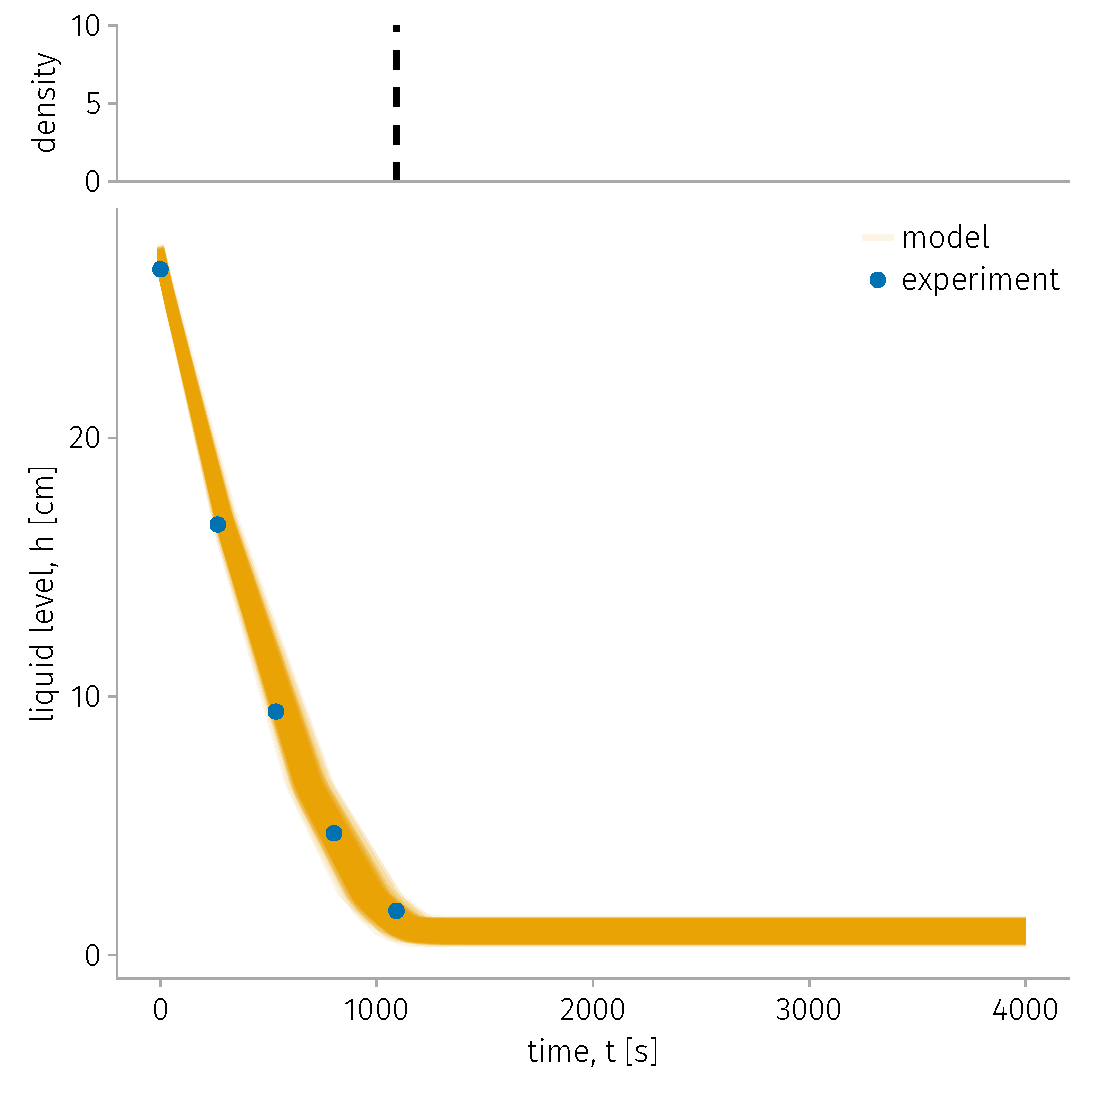
\includegraphics[width=0.5\textwidth]{../test.pdf}
    \caption{
      \textbf{Testing the calibrated forward model.}
      (Bottom) Comparison between water level time series data from a replicate tank drainage experiment and water level trajectories predicted by the calibrated forward model. 
      (Top) Distribution of predicted emptying times.
      } \label{fig:test}
\end{figure}

\subsection{Phase II: Bayesian inference of the shape of a solid inside the tank} \label{sec:phaseII}
Finally, we exploit our calibrated model to infer the shape of an exogenous, stationary, heavy solid (incapable of holding water itself) inside of our tank from water level time series data as it drains.
Our objective is to obtain the posterior distribution of $\mathbf{A}$ characterizing the cross-sectional area of the solid as a function of height, $\alpha(h; \mathbf{A})$.

\subsection{Experimental setup}
We set up a tank drainage experiment by:
(i) placing a solid object---a large, capped, glass bottle filled with water [so it sinks]---inside of the tank, which remains stationary;
(ii) filling the tank to an initial water level (measured by the level strip) of $h_{0, \text{obs}}=26.49$\,cm. 
See Fig.~\ref{fig:tank_w_bottle}.


\subsection{Prior distributions}
Before allowing the tank to drain, we express our prior knowledge and beliefs about the inputs and parameters. 
%Our prior distribution for (i) the initial water level $H_0$ is informed by the initial water level measurement; (ii) the parameter vector $\boldsymbol \Theta$ and measurement noise variance $\Sigma^2$ is informed by the model calibration phase; and (iii) the object area $\mathbf{A}$ (a) is diffuse, to entertain a large range of possible object shapes in the tank, and (b) promotes a smooth function $\alpha(h)$. Fig.~\ref{fig:prior_area} displays samples from the prior distribution for the object shape vector $\mathbf{A}$. 
% Below, we express our knowledge and beliefs about the inputs and parameters, before allowing the tank to train and collecting water level time series data, by constructing a prior probability density $\pi_{\text{pr}}(h_0, \boldsymbol \alpha, \boldsymbol \theta, \sigma^2)$. 

% \vspace{-\baselineskip}
\subparagraph{The parameter vector and measurement noise variance.}
Adopting the adage ``yesterday's posterior is today's prior'' \cite{calvetti2010subjective}, 
our multi-variate Gaussian posterior distribution of the parameter vector $\boldsymbol \Theta$ and noise variance $\Sigma^2$ in eqn.~\ref{eq:post_theta_sigma} from model calibration now serves as our prior distribution.
Thereby, we exploit our \emph{calibrated} model for this reconstruction problem.
(We assume the solid in the tank does not affect the discharge coefficient.)

\vspace{-\baselineskip}
\subparagraph{Initial water level.} We again impose an informative prior distribution on the initial water level based on the initial reading of the water level sensor:
\begin{equation}
	H_0 \mid \Sigma = \sigma \sim \mathcal{N}(h_{0, \text{obs}}, \sigma^2).
\end{equation}

\vspace{-\baselineskip}
\subparagraph{Shape of the exogenous solid.}
We adopt the principle of indifference and impose a diffuse prior over the size of the solid in the tank, but impose smoothness on the cross-sectional area of the solid as a function of height to counter instability in the solution to this inverse problem \cite{groetsch1993inverse}. 
By imposing a diffuse prior on the solid's size, we allow the water level time series data to ``speak for itself'' about the solid's size.
Specifically, we impose a uniform distribution on the square root of the area of the bottom base of the solid, $A_0$ (the random variable representing $\alpha(0)$)
\begin{equation}
	\sqrt{A_0} \mid A_b=a_b \sim \mathcal{U}(0, \sqrt{a_b}).
\end{equation}
Ie., we believe 
(i) the area of the solid's bottom base can span from zero (corresponding to the lack of an exogenous solid) to the area of tank's bottom base $a_b$ (corresponding to the largest solid that can fit in the tank) and
(ii) the effective radius of the solid is uniformly distributed.
For the smoothness prior \cite{calvetti2018inverse}, we sequentially correlate the solid's effective radius at the sequence of heights: 
\begin{equation}
 \sqrt{A_i} - \sqrt{A_{i-1}} \sim \mathcal{N}(0, \gamma^2) \text{ for } i \in \{1, ..., n\}.
\end{equation} 
The zero mean Gaussian distribution on the difference in the effective radius of the solid at two adjacent heights means we expect the function $\sqrt{\alpha(h)}$ to be locally flat and change slowly. 
The variance hyperparameter $\gamma^2$ controls the degree to which we promote smoothness in $\sqrt{\alpha (h)}$ (smaller $\gamma^2$ promotes more smoothness). 
Finally, for physicality, we also truncate each random variable $A_i$ so it falls within zero to the area of the tank at that height.

\paragraph{Visualization of the prior.}
Fig.~\ref{fig:prior_area} displays samples of our prior distribution on the solid's area as a function of height---by sampling a vector $\mathbf{A}$ from the prior then constructing $\alpha(h)$ from cubic monotonic interpolation. The square root of the area of the tank is shown for perspective. 
Our prior distribution encodes a uniform distribution over the effective average radius of the solid in the tank, but promotes a smoothly changing area as a function of height. 
%  This is a visualization of our beliefs about the shape of the object in the tank before water level time series data from the ``object scan'' are collected and considered against the forward model.

\subsection{Water level time series data from a tank-drainage experiment}
At time $t:=0$, we allow our tank containing the exogenous solid to drain of water. Fig.~\ref{fig:posterior_object} shows the time series data of the water level \thedata obtained from our level sensor.

\subsection{Posterior distribution}
Again, we employ NUTS to obtain samples from the posterior $\pi_{\text{post}}(h_0, \boldsymbol \alpha, \boldsymbol \theta, \sigma^2 \mid \thedatanomath)$. 
%Via Bayes's theorem in , the posterior distribution $\pi_{\text{post}}(h_0, \boldsymbol \alpha, \boldsymbol \theta, \sigma^2 \mid \thedatanomath)$ follows from (i) prior probability density $\pi_{\text{pr}}(h_0, \boldsymbol \alpha, \boldsymbol \theta, \sigma^2)$---informed for $H_0$, $\boldsymbol \Theta$, and $\Sigma^2$ and diffuse but smooth for $\mathbf{A}$---and (ii) tank drainage data \thedata, from which we construct the likelihood function in eqn.~\ref{eq:like}, the posterior distribution $\pi_{\text{post}}(h_0, \boldsymbol \alpha, \boldsymbol \theta, \sigma^2 \mid \thedatanomath)$ follows from Bayes's theorem in eqn.~\ref{eq:post}. 
%We employ the MCMC sampler, NUTS, to obtain samples $\{(h_{0,i}, \boldsymbol \alpha_i, \boldsymbol \theta_i, \sigma^2_i\}$ from the posterior distribution. 

Fig.~\ref{fig:posterior_area} shows posterior samples of the square root of the area of the solid as a function of height---the BSI solution to the reconstruction problem. 
For comparison, we also show (i) the bottle's [roughly-] ground-truth area at different heights inferred from our length-measurements of its circumference and (ii) for context, posterior samples of the tank's area as a function of height. First, the posterior of the solid's shape exhibits much lower variance than the prior in Fig.~\ref{fig:prior_area}---reflecting the information the water level time series data provided about the solid's shape. 
Second, the posterior of the solid's shape agrees reasonably well with the measured area of the solid (mean residual radius: 0.35\,cm; mean bottle radius 3.2\,cm), but a little bias is present in $h\in[15, 20]$\,cm.
Third, note the variance in the posterior over the solid's area in $h<h_o$ and $h>h_{\text{max}}$ is larger than in $h_o < h < h_{\text{max}}$. This reflects the impossibility for the water level data to provide information about the solid's area where the water was unable to ``scan'' the solid. 
For $h<h_o$ and $h>H$, the smoothness prior restricts the variance of the predicted area---essentially, extrapolating. 

Overall, Fig.~\ref{fig:posterior_area} illustrates our ability to infer the shape of a solid inside a draining tank with quantified uncertainty---using (i) a calibrated dynamic model of the water level in the tank and (ii) water level time series data over the process of draining. % The key idea is that the water ``scans'' the object's area as a function of height as it drops.

As a posterior predictive check, Fig.~\ref{fig:posterior_object} displays samples of liquid level trajectories \themodel from the posterior distribution, which match the water level time series data \thedata reasonably well (mean absolute residual: 0.35\,cm). 

\begin{figure}[h!]
    \centering
        \begin{subfigure}[b]{0.3\textwidth}
    	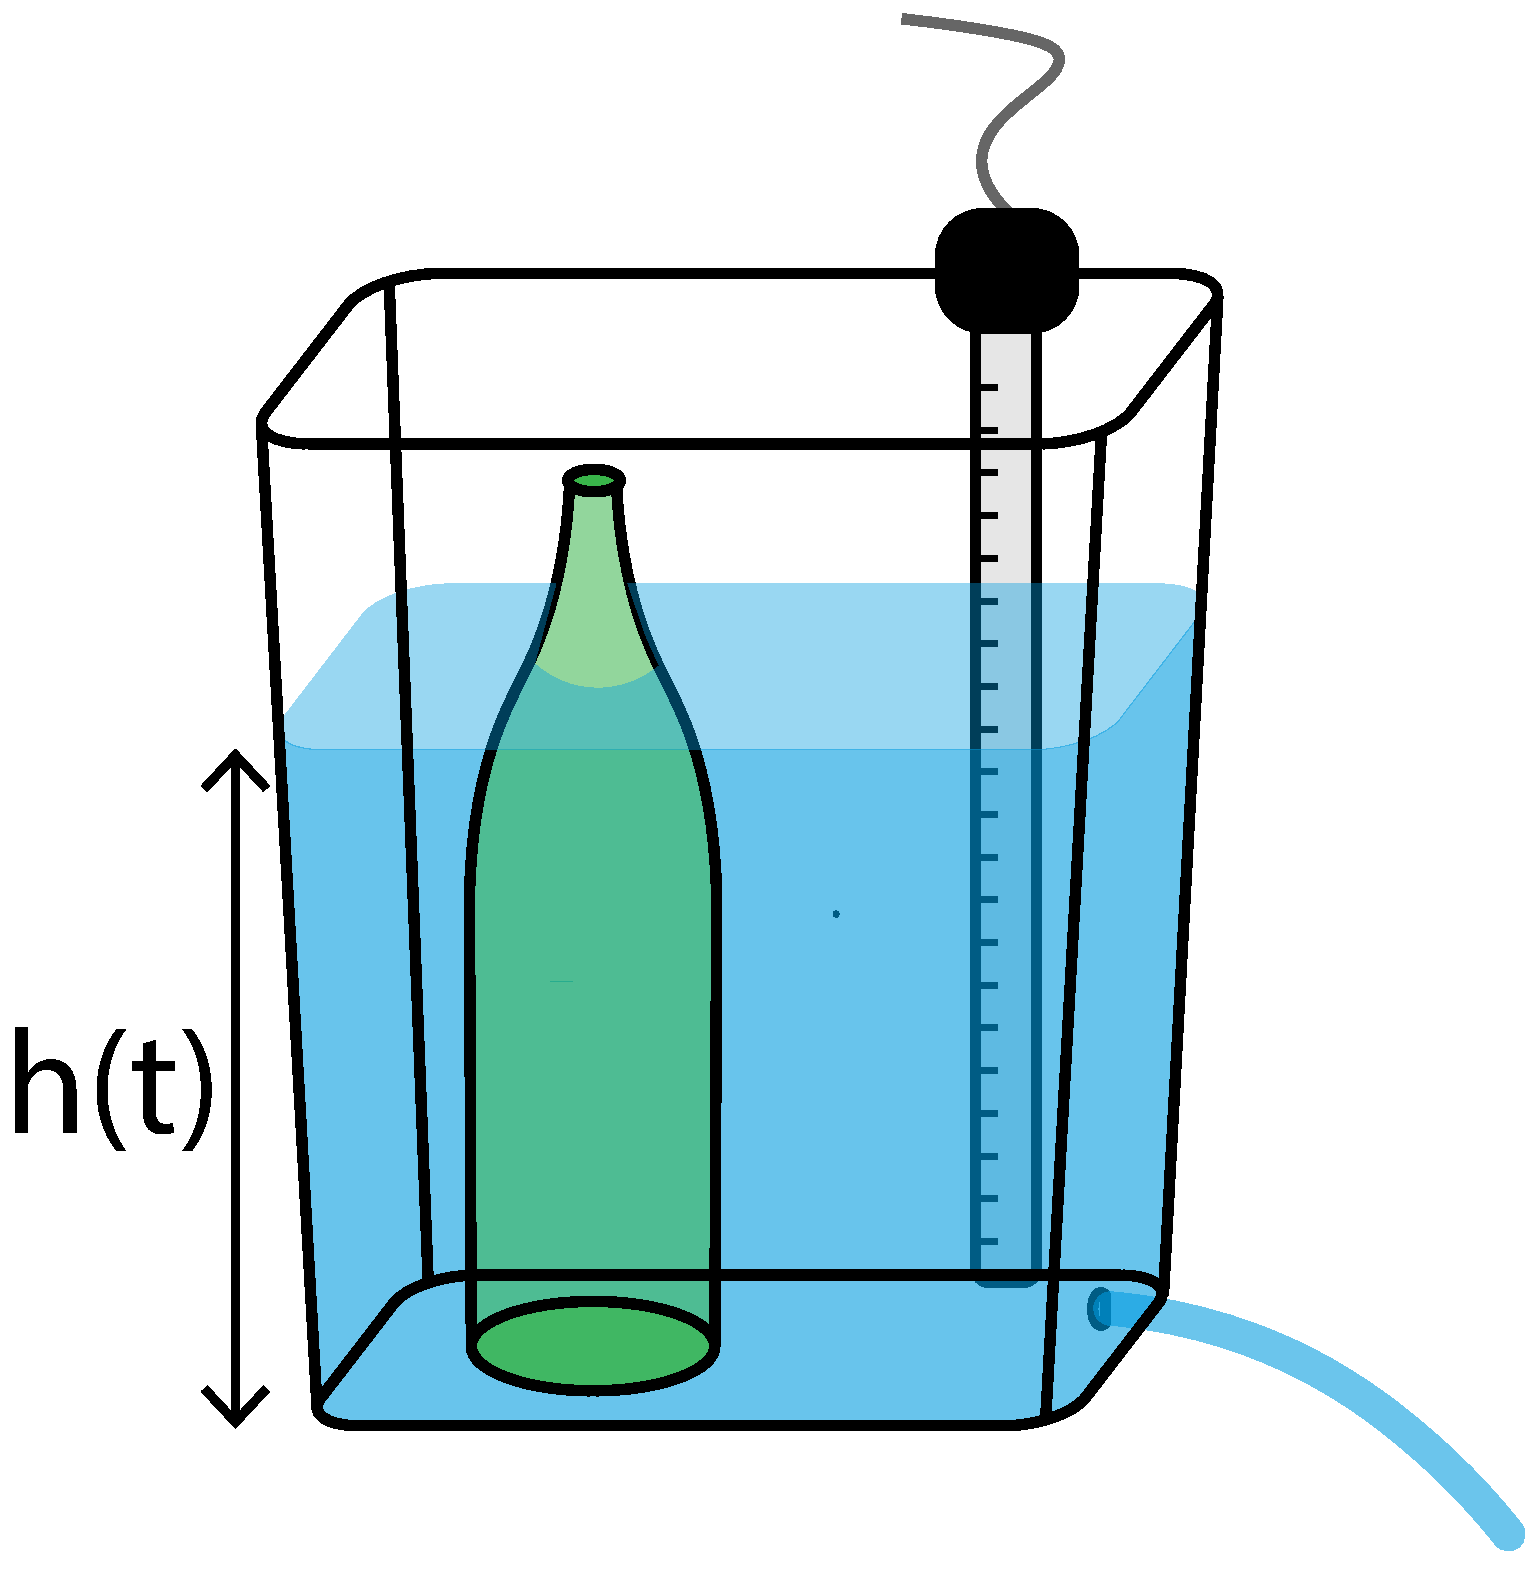
\includegraphics[width=\textwidth]{../tank_geometry/tank_w_bottle.pdf}
	\caption{Experimental setup} \label{fig:tank_w_bottle}
    \end{subfigure}
     \begin{subfigure}[b]{0.49\textwidth}
    	\includegraphics[width=\textwidth]{../prior_area.pdf}
	\caption{Prior distribution} \label{fig:prior_area}
    \end{subfigure}
    
     \begin{subfigure}[b]{0.49\textwidth}
    	\includegraphics[width=\textwidth]{../posterior_object.pdf}
	\caption{Data \& posterior distribution} \label{fig:posterior_object}
    \end{subfigure}
    \begin{subfigure}[b]{0.49\textwidth}
    	\includegraphics[width=\textwidth]{../posterior_area.pdf}
	\caption{Posterior distribution} \label{fig:posterior_area}
    \end{subfigure}
    \caption{
      \textbf{Reconstructing the shape of an exogenous solid in the draining tank.} 
      (a) We fill our tank, containing a heavy glass bottle, with water, then, at $t=0$, allow it to drain through the orifice in its side.
      (b) Samples of the square root of the solid's area as a function of height from the prior (orange lines), along with the square root of the area of the tank (gray), depicted assuming radial symmetry.
      (c) Time series data from the tank drainage experiment and samples of water level trajectories from the posterior.
      (d) Samples of the square root of the solid's inferred area as a function of height from the posterior distribution (orange lines) compared with held-out, direct measurements (points) and the tank's area (gray).
      }
\end{figure}

\section{Conclusions and Discussion}
We demonstrated our ability to reconstruct, with quantified uncertainty, the cross-sectional area of a heavy, exogenous solid (incapable of holding water) inside a tank from (i) a calibrated dynamic model of the liquid level in the tank as it drains through a small orifice and (ii) measurements of the liquid level in the tank over time as it drains.
First, we constructed, Bayesian-calibrated, and tested a forward model for the dynamics of the liquid level in our tank draining of water.
The calibrated model predicted the liquid level trajectory in our tank in a replicate experiment with a mean absolute residual of 0.28\,cm.
Then, we exploited our Bayesian-calibrated forward model to reconstruct the shape of an exogenous, heavy solid (a bottle) inside our draining tank using water level time series data. 
Essentially, the water ``scanned'' the area of the solid as a function of its height as the tank drained. 
The posterior distribution of the bottle's area as a function of height agreed reasonably well with our [more] direct measurements of its area, with $\sim 10$\% reconstruction error over the bottle's radius. 
% In conclusion, a forward model of the dynamics of the liquid level in a draining tank containing an exogenous solid, a probabilistic measurement model of the liquid level sensor, and liquid level time series data during the process of draining together allow us to reconstruct the area of the exogenous solid as a function of height with quantified uncertainty via Bayesian statistical inversion. 

Our methodology herein could be employed throughout engineering and the applied sciences to infer the shape of an exogenous solid inside of an opaque or underground \cite{gephart2010short} liquid-holding tank in a non-destructive manner, provided we have access to liquid level measurements.
In a similar manner, one could also infer the height and/or porosity of small, heavy solid particles (e.g. gravel, sand) packed into a liquid holding tank \cite{guellouz2020estimation}.

\paragraph{Can we infer the precise geometry of a solid in an opaque, draining tank?}
We inhibited our ambition to reconstruct the geometry of an exogenous solid inside a draining tank from its liquid level over time by settling for its area as a function of height; determining the precise geometry of the solid is impossible because the dynamics of $h(t)$ depend solely on the area of the solid as a function of height (see eqn.~\ref{eq:forward_model})---and, there are multiple non-congruent solids with an identical area as a function of height. We speculate that, by conducting multiple tank-draining experiments with the tank tilted and held at different angles, we may be able to reconstruct the precise geometry of the solid in the tank. The key idea is that two non-congruent solids with an identical area as a function of height may exhibit different areas as a function of height when tilted; thus, they can be distinguished by tilting the tank. A complication is that gravity could cause the shape to rotate when the tank is tilted. 


\paragraph{Remarks.} (1) We could have calibrated our forward and measurement models using data from a tank drainage experiment where the tank \emph{did} contain an exogenous solid, provided the area of the solid as a function of height were known with some certainty. (2) If we knew the solid's shape belonged to a certain category (eg.\ a right circular cone), we could have parameterized its area as a function of height with fewer variables (eg.\ height and base radius). 

\paragraph{Extensions.}
(1) Our forward model of the dynamics of the liquid level in an \emph{open-top} tank, containing a \emph{solid}, draining of liquid through a \emph{small} orifice in its side \emph{without} additional input/output of liquid could be extended to handle inverse problems concerning
(a) closed tanks, where the air pressure in the headspace is not constant and atmospheric during draining; 
(b) larger orifices, where Torricelli's law does not hold and perhaps the liquid at the top does not remain flat (necessitating modeling of flow streamlines as in Refs.~\cite{mathew2014numerical,sakri2017numerical});
(c) additional inputs/outputs of liquid by adding source/sink terms; 
(d) Mariotte's bottle \cite{kirevs2006mariotte}; and/or
(e) a flexible object compressible by hydrostatic pressure, such as a balloon \cite{muller2004rubber}. 
(2) During Bayesian model calibration, a model discrepancy \cite{brynjarsdottir2014learning,kennedy2001bayesian} function could capture any bias---i.e., a difference between the true dynamics of the liquid level in the tank and the model $h(t; h_0^*,  \boldsymbol \alpha^*, \boldsymbol \theta^*)$ with the true/best-fit (indicated by $*$) initial water level, solid geometry, and parameters.
% In other words, we assume our forward model is capable of capturing the true liquid level dynamics in the tank without bias.
(3) Finally, another interesting inverse problem pertaining to a draining tank is time reversal: infer the initial water level from measurement(s) of the water level at later times.

\paragraph{Other geometric inverse problems.}
Examples of other geometric inverse problems, where the unknown is a geometric shape \cite{ameur2004level,burger2001level,harbrecht2013numerical}, include inferring the shape and location of cracks in a solid \cite{nishimura1991boundary}, fouling on the inner wall of a pipe \cite{chen2011inverse}, mines underground \cite{delbary2007inverse,lopez2003detection}, scattering objects like submarines \cite{yaman2013survey} underwater \cite{buchanan2004marine}, and inclusions or cavities inside thermal conductors \cite{wang2018numerical,nakamura2015reconstruction}
 from boundary measurements; inferring the shape of obstacles in blood vessels from flow measurements \cite{aguayo2021distributed,nolte2022inverse}; and inferring the shape of a membrane from the sound it produces when it vibrates \cite{kac1966can}.



\subsubsection*{Data and code availability} The raw liquid level time series data and Julia code to reproduce our results are available at \url{github.com/SimonEnsemble/tank_inverse_problem}.


\enlargethispage{20pt}

\ack{CMS acknowledges support from the Intel Corporation through their Mindshare Program - Broadening Participation in Science and Engineering Higher Education. 
GF acknowledges ARMI for funding. 
Hat tips to Brian Wood for helpful discussions about the possibility to infer the precise shape of the solid in the tank by tilting it; Adrian Henle for feedback on our manuscript; and Axel Rodriguez for help articulating the condition for a solid to be incapable of holding water.}


\vskip2pc


\bibliographystyle{RS} %%%% .BST file

\bibliography{refs} %%%%% .Bib file

\end{document}
